\chapter{Methodology}
\label{ch:methodology}
\label{ch:architecture}

This chapter explains how the proposed process-evaluation approach is defined, implemented, and evaluated. It begins by setting out the state/action/trace notation used throughout the chapter (\S\ref{sec:methodology-notation}). It then defines the process-quality score (\S\ref{sec:methodology-score}--\S\ref{sec:methodology-cleanliness}) and describes the event-capture, shadow-repository, and metrics infrastructure that supplies the data for that score (\S\ref{sec:arch-events}--\S\ref{sec:arch-metrics}). Next, it introduces the divergence-point detector (\S\ref{sec:methodology-detector}), the Eclipse JDT substrate used to construct alternatives (\S\ref{sec:arch-jdt}), the per-kind alternative trajectory synthesisers (\S\ref{sec:methodology-reorder}--\S\ref{sec:methodology-hygiene}), and the validator used to check that each alternative still reaches the same end state (\S\ref{sec:methodology-validator}). The chapter then describes the overall system architecture and offline/replay pipeline (\S\ref{sec:arch-overview}--\S\ref{sec:methodology-phases-split}), followed by the participant dashboard (\S\ref{sec:arch-dashboard}). Finally, it defines the evaluation methodology used in Chapter~\ref{ch:results}: the score-formula sensitivity and ablation design (\S\ref{sec:methodology-score-eval}), the 45-session dataset and labelling protocol (\S\ref{sec:methodology-rater}), and the divergence-detector evaluation protocol (\S\ref{sec:methodology-detector-eval}).

\section{Formal definitions and notation}
\label{sec:methodology-notation}

The formal definitions in this section build on the state/action/trace framing from \S\ref{sec:def-framing}. A refactoring trajectory is a sequence
\[
\tau = (s_0, a_0, s_1, a_1, \ldots, a_{T-1}, s_T),
\]
where each $s_t$ is a code snapshot and each $a_t$ is a developer action that turns $s_t$ into $s_{t+1}$. Actions are either IDE-supported refactoring operations or manual edits; in practice a single action can carry both a structured refactoring spec (recovered by RefactoringMiner~\cite{alikhanifard2025rminer}) and some leftover unstructured edits. We treat this as one action with two parts rather than two separate actions.

The tool evaluates a trajectory by producing an \emph{analysis report}. For a trajectory $\tau$, this report is written as the tuple $(\tau, \mathcal{M}, \mathcal{D}, \mathcal{A})$, where:
\begin{itemize}
  \item $\mathcal{M} = \{m_0, m_1, \ldots, m_T\}$ is the set of metrics collected for the states in the trajectory. Each $m_t$ contains the cleanliness sub-score $C(s_t)$ and the raw signals used to compute it, including PMD violations, CPD duplications, Chidamber--Kemerer measures, build/test outcomes, the action's refactoring spec, and commit and test event metadata.
  \item $\mathcal{D}$ is the set of divergence points the detector emits for $\tau$ (\S\ref{sec:methodology-detector}).
  \item $\mathcal{A}$ is the set of alternative reference trajectories synthesised at those divergence points (\S\ref{sec:methodology-reorder} onwards). Each $\tau^\ast \in \mathcal{A}$ is represented in the same way as the observed trajectory, which allows both trajectories to be scored using the same process-quality score.
\end{itemize}

The process-quality score $J(\tau)$ is computed over the full trajectory using $\mathcal{M}$, and is the focus of \S\ref{sec:methodology-score}--\S\ref{sec:methodology-weights}. Table~\ref{tab:methodology-notation} summarises the notation used throughout the chapter.

\begin{table}[htbp]
\centering
\small
\begin{tabular}{ll}
\hline
\textbf{Symbol} & \textbf{Meaning} \\
\hline
$\tau = (s_0, a_0, s_1, \ldots, a_{T-1}, s_T)$ & Refactoring trajectory \\
$s_t$ & State (code snapshot) at step $t$ \\
$a_t$ & Action at step $t$ (IDE refactor or manual edit) \\
$J(\tau)$ & Process-quality score, clamped to $[0, 100]$ \\
$C(s)$ & Cleanliness sub-score of state $s$ \\
$\Delta C(\tau) = C(s_T) - C(s_0)$ & Cleanliness gain across trajectory \\
$\beta = 50$ & Baseline anchor in the process score \\
$W_{\textsc{x}}$ & Process-score weight for term \textsc{x} \\
$r_b,\ r_{st},\ r_{mi}$ & Laplace-smoothed rate terms (broken, skip-tests, manual-when-IDE) \\
$n_{cg}(\tau)$ & Commit-gap event count \\
$\sigma_l(\tau)$ & Step-savings bonus for alternative trajectories \\
$\mathrm{DP}$ & Divergence point \\
$\tau^{\ast}$ & Alternative reference trajectory \\
$\mathcal{K}$ & Divergence-kind set $= \{\emph{Ordering}, \emph{Manual-Refactor}, \emph{Rework}, \emph{Hygiene}\}$ \\
\hline
\end{tabular}
\caption{Notation used throughout the methodology chapter.}
\label{tab:methodology-notation}
\end{table}

\section{Computing the process score}
\label{sec:methodology-process-score-section}

This section defines the process score $J(\tau)$ and the cleanliness sub-score used inside it (\S\ref{sec:methodology-score}--\S\ref{sec:methodology-cleanliness}). It then describes how the tool captures events, reconstructs shadow repositories, and calculates the per-checkpoint metrics needed to compute the score (\S\ref{sec:arch-events}--\S\ref{sec:arch-metrics}).

\subsection{The process score}
\label{sec:methodology-score}

The process score $J(\tau)$ combines seven weighted terms across the trajectory and clamps the result to a $[0, 100]$ range so trajectories of different lengths can be compared on the same scale:
\begin{equation}
J(\tau) = \mathrm{clip}_{[0,100]}\Big(\beta + W_{\textsc{g}}\,\Delta C(\tau) - W_{\textsc{b}}\,r_b(\tau) - W_{\textsc{st}}\,r_{st}(\tau) - W_{\textsc{mi}}\,r_{mi}(\tau) - W_{\textsc{cg}}\,n_{cg}(\tau) - W_{\textsc{lag}}\,\ell(\tau) + W_{\textsc{l}}\,\sigma_l(\tau)\Big)
\label{eq:process-score}
\end{equation}
where:
\begin{itemize}
  \item $\beta = 50$ is the baseline. A trajectory with no cleanliness gain and no process penalties scores 50.
  \item $\Delta C(\tau) = C(s_T) - C(s_0)$ is the cleanliness gain from start to end (\S\ref{sec:methodology-cleanliness}).
  \item $r_b(\tau) = b_{\mathrm{ms}}(\tau) / e_{\mathrm{ms}}(\tau)$ is the fraction of wall-clock time for which the build or test suite was broken.
  \item $r_{st}(\tau)$ and $r_{mi}(\tau)$ are event-rate penalties. They use Laplace smoothing, $r_\bullet(\tau) = (k + 1) / (n + 2)$, where $k$ is the number of penalised events and $n$ is the number of opportunities. If no relevant events have occurred yet, the term is set to zero.
  \item $n_{cg}(\tau)$ counts commit-gap events. One event is recorded for each stretch of at least six green-refactor checkpoints between user commits.
  \item $\ell(\tau) \in [0, 1]$ measures intermediate-cleanliness lag. It is the per-checkpoint running mean of $\max\!\big(0,\; C(s_T) - C(s_i)\big)$ over the trajectory, in scalar cleanliness units. This term is positive while the trajectory remains below its final cleanliness level, so it penalises paths that spend longer in degraded intermediate states.
  \item $\sigma_l(\tau)$ is a step-savings bonus for synthesised alternatives. It contributes only when $\tau$ is an alternative trajectory that reaches the same end state in fewer steps than the observed user trajectory.
\end{itemize}

Three design choices shape this formula. First, the penalty for a broken build or test suite must be larger than any plausible single-step cleanliness gain. This prevents a trajectory from being rewarded overall for improving structure while temporarily breaking correctness. The weight ordering $W_{\textsc{b}}\!:\!W_{\textsc{st}}\!:\!W_{\textsc{cg}} = 28\!:\!14\!:\!7$ encodes this priority in \S\ref{sec:methodology-weights}. Second, Laplace smoothing prevents the event-rate terms from being dominated by one early event on a very short trajectory. Third, clamping the score to $[0, 100]$ makes trajectories easier to compare, but it also introduces saturation: when a user's trajectory is already close to 100, the improvement available to a higher-scoring alternative is compressed by the ceiling. The sensitivity experiment in \S\ref{sec:results-sensitivity} treats this as a known limitation of the score formula.

The score is intended as a consistent and literature-grounded way to compare refactoring trajectories, not as a uniquely correct measure of process quality. There is no held-out ground truth for ``true refactoring-trajectory quality'' against which the weights could be calibrated directly. The empirical evidence in Chapter~\ref{ch:results}, including the sensitivity sweep, ablation study, and inter-rater agreement analysis, therefore evaluates robustness, term importance, and classifier accuracy rather than proving that the chosen weights are optimal.

\subsection{Process-score weights}
\label{sec:methodology-weights}

Table~\ref{tab:methodology-weights} lists the seven weights used in Equation~\eqref{eq:process-score} and summarises the literature behind each one. This section explains why the terms are included. Their empirical effect on the ranking is examined later through the ablation analysis in \S\ref{sec:results-ablation}, which tests all $2^7 = 128$ weight subsets per fixture and reports both solo and leave-one-out recovery against the full formula.

\begin{table}[htbp]
\centering
\small
\begin{tabular}{l r p{0.52\textwidth}}
\hline
\textbf{Term} & \textbf{Weight} & \textbf{Cited justification} \\
\hline
$W_{\textsc{g}}$ (gain)        & 50 & Cedrim et al. 2017~\cite{cedrim2017refactoring}; Paix{\~a}o et al. 2017~\cite{paixao2017balancing} \\
$W_{\textsc{b}}$ (broken)      & 28 & Paix{\~a}o et al. 2017~\cite{paixao2017balancing}; Gautam et al. 2025~\cite{gautam2025refactorbench} (FM \#2) \\
$W_{\textsc{st}}$ (skip-tests) & 14 & Murphy-Hill et al. 2009~\cite{murphyhill2009howrefactor} \\
$W_{\textsc{mi}}$ (manual)     & 11 & Negara et al. 2013~\cite{negara2013manualautomated}; Vakilian et al. 2012~\cite{vakilian2012usedisuse} \\
$W_{\textsc{l}}$ (length)      & 11 & Harman \& Tratt 2007~\cite{harman2007pareto}; Mohan \& Greer 2019~\cite{mohan2019manyobjective} \\
$W_{\textsc{lag}}$ (lag)       & 11 & Cunningham 1992~\cite{cunningham1992wycash}; Kruchten et al. 2012~\cite{kruchten2012technicaldebt}; Cedrim et al. 2017~\cite{cedrim2017refactoring}; Paix{\~a}o et al. 2017~\cite{paixao2017balancing} \\
$W_{\textsc{cg}}$ (commit-gap) & 7  & Tao \& Kim 2015~\cite{taokim2015partitioning}; Di Biase et al. 2019~\cite{dibiase2019decomposition}; Herzig \& Zeller 2013~\cite{herzig2013tangled}; Kudrjavets et al. 2022~\cite{kudrjavets2022small} \\
\hline
\end{tabular}
\caption{Weights used in Equation~\eqref{eq:process-score} and the literature supporting each term. The empirical contribution of each term is examined in the ablation analysis of \S\ref{sec:results-ablation}.}
\label{tab:methodology-weights}
\end{table}

The rest of this section explains each weight in turn. For two terms, $W_{\textsc{mi}}$ and $W_{\textsc{cg}}$, the literature supports the underlying concern but does not give numerical evidence for how large those penalties should be. Those limitations are noted in the relevant paragraphs.

\paragraph{$W_{\textsc{g}}$ (gain, 50).}
This is the main positive term in the score: each unit of cleanliness gain at the end of the trajectory adds 50 to $J(\tau)$. Cedrim et al.~\cite{cedrim2017refactoring} found that refactoring often leaves structural metrics unchanged or slightly worse, so improvement should be rewarded explicitly rather than assumed. Paix{\~a}o et al.~\cite{paixao2017balancing} model the balance between disruption and improvement as something developers actively manage, which motivates treating cleanliness gain and process penalties as competing parts of the same score.

\paragraph{$W_{\textsc{b}}$ (broken, 28).}
This is the largest single penalty term. Paix{\~a}o et al.~\cite{paixao2017balancing} show that developers place substantial value on avoiding disruptive intermediate states, even when doing so means giving up roughly a quarter of the available metric improvement. The penalty is time-weighted rather than binary: $r_b(\tau) = b_{\mathrm{ms}} / e_{\mathrm{ms}}$, so a brief broken state is penalised less than a long one. The numerator $b_{\mathrm{ms}}$ counts only wall-clock time during which the build or tests are failing, rather than total refactoring time.

Time-weighting also makes the term less sensitive to how finely the trajectory is sampled. The state/action/trace framing in \S\ref{sec:methodology-notation} allows a state to be a commit, an IDE event, or a developer-defined checkpoint. A binary count of broken states would vary substantially across those choices, whereas wall-clock time spent broken is independent of the sampling rate. This choice is also consistent with Gautam et al.'s RefactorBench analysis~\cite{gautam2025refactorbench}: their failure-mode~\#2 shows that rejecting every intermediate broken state can hurt LM-agent performance, because some broken intermediates are necessary during multi-file edits. The weight is therefore set high enough that a plausible single-step cleanliness gain, $W_{\textsc{g}}\,\Delta C$, cannot outweigh leaving the build or tests broken.

\paragraph{$W_{\textsc{st}}$ (skip-tests, 14).}
This term penalises 60-second refactoring windows that finish without a test run. The window size follows Murphy-Hill et al.~\cite{murphyhill2009howrefactor}, whose study of real refactoring practice shows that developers tend to run tests after batches of changes rather than after every individual edit. The weight is set to half of $W_{\textsc{b}}$: skipping tests is weaker evidence of process damage than an observed broken state, but it still indicates reduced feedback during the refactoring process.

\paragraph{$W_{\textsc{mi}}$ (manual-when-IDE, 11).}
This term penalises steps where the developer performs a refactoring manually even though the IDE could have applied the same transformation automatically. Mens \& Tourw{\'e}~\cite{mens2004survey} note that IDE refactoring tools apply static precondition checks that manual edits may bypass, making the automated route safer in many cases. At the same time, manual refactoring is common: Negara et al.~\cite{negara2013manualautomated} found that, across 23 developers and 5,371 refactorings, developers often performed refactorings by hand even when an automated equivalent was available. Vakilian et al.~\cite{vakilian2012usedisuse} also show that automated refactorings can be misused, so the term is treated as a graded penalty rather than a hard rule.

No published study that we are aware of directly measures the fault-rate gap between manual and IDE refactoring, so this weight is not fitted to such data. Instead, it follows the severity ordering set out above. The ablation analysis in \S\ref{sec:results-ablation} shows that \texttt{manualIde} is one of the three largest single-term contributors by sum-over-sum recovery to session-wide divergence-point magnitude, alongside \texttt{length} and \texttt{broken} (Table~\ref{tab:results-ablation-solo}), and the sensitivity sweep in \S\ref{sec:results-sensitivity} indicates that the ranking is robust to perturbations of this weight.

\paragraph{$W_{\textsc{l}}$ (length, 11).}
This is a positive term rather than a penalty. It increases $J(\tau)$ only for alternative trajectories that reach the same end state as the observed user trajectory in fewer steps. Search-based refactoring work treats the number of refactoring operations as an optimisation objective alongside quality \cite{harman2007pareto,mohan2019manyobjective}, and later many-objective work continues this by trading effort against code-quality objectives \cite{cortellessa2023manyobjective}. The observed user trajectory is not penalised for length, since a longer path may reflect a larger or more complex task rather than a worse process. The term therefore rewards shorter valid alternatives without treating every long trajectory as poor.

\paragraph{$W_{\textsc{lag}}$ (lag, 11).}
This term penalises trajectories that spend time in a worse cleanliness state before reaching their final value. The gain term $W_{\textsc{g}}\,\Delta C$ only compares the start and end states, so two trajectories receive the same gain score if they finish with the same cleanliness improvement, even if one cleans up early and the other leaves the code degraded until the end. The lag term adds a cost for this delay.

The motivation is similar to technical debt. Cunningham's debt metaphor~\cite{cunningham1992wycash} and Kruchten et al.'s later formalisation~\cite{kruchten2012technicaldebt} both treat degraded code as something that becomes more costly the longer it remains. Cedrim et al.~\cite{cedrim2017refactoring} give empirical support for applying this idea to refactoring sequences: they show that intermediate states can degrade structural metrics relative to the start, even when the final result is an improvement. The lag term therefore penalises time spent below the trajectory's final cleanliness target, rather than only measuring the endpoint gap.

The weight is set to $11$, the same as $W_{\textsc{l}}$ and $W_{\textsc{mi}}$, and half of the broken-state penalty $W_{\textsc{b}}$, following the severity ordering in \S\ref{sec:methodology-weights}. Since $\ell \in [0, 1]$, the maximum lag penalty is $11$ points, which keeps it smaller than the maximum gain credit of $50$. The ablation results give the strongest support for this term in the \emph{Ordering} category: \S\ref{sec:results-ablation} reports its solo magnitude-recovery, and \S\ref{sec:results-divergence} shows that the number of \emph{Ordering} divergence-points where the synthesised alternative beats the user's trajectory rises from 4 to 10 of 24 once $W_{\textsc{lag}}$ is included.

\paragraph{$W_{\textsc{cg}}$ (commit-gap, 7).}
This term penalises long runs of green checkpoints, where the refactoring checks and tests pass, without a commit in between. The aim is to capture a small process cost: when several valid steps are left bundled together, the resulting change is harder to review, explain, or roll back than if the work had been split into smaller confirmed units.

The evidence comes from work on decomposing composite changes. Tao \& Kim~\cite{taokim2015partitioning} report that separated commits let reviewers inspect changes more effectively in the same amount of time. Di Biase et al.'s controlled experiment~\cite{dibiase2019decomposition} points in the same direction: decomposed changes produced fewer comments that incorrectly marked correct code as defective (1 rather than 6, $p=0.03$). Tangled commits can also make later defect attribution less reliable~\cite{herzig2013tangled}.

This is deliberatley a narrow claim. Kudrjavets et al.~\cite{kudrjavets2022small} find no correlation between PR size and time-to-merge across 1.25M PRs in ten languages, so the term is not meant to capture merge speed. It is instead used as a smaller hygiene signal for review comprehensibility and rollback locality. Because no published study that we are aware of directly links commit cadence during refactoring to these costs, the weight is not fitted to data. The ablation results are consistent with this lower-severity role: \texttt{commitGap} recovers non-zero session-set magnitude on its own (sum/sum $0.126$), and removing it changes the ranking (mean $\tau=0.926$) while leaving most total magnitude intact (sum/sum $0.892$).

\subsection{The cleanliness sub-score}
\label{sec:methodology-cleanliness}

The cleanliness sub-score $C(s)$ in Equation~\eqref{eq:process-score} gives each codebase state a normalised quality value in $[0, 100]$. It is built from six signals rather than one, following the argument in \S\ref{sec:smells-metrics} that individual quality measures are noisy and context-dependent. Combining several signals makes the score less dependent on any single metric. Table~\ref{tab:methodology-cleanliness} lists the six sub-signals, the source used to justify each one, and how each value is computed.

\begin{table}[htbp]
\centering
\small
\begin{tabular}{l r p{0.36\textwidth} p{0.24\textwidth}}
\hline
\textbf{Sub-metric} & \textbf{Weight} & \textbf{Cited basis} & \textbf{Computation source} \\
\hline
Cognitive complexity & 1.0 & Campbell 2018~\cite{campbell2018cognitive}; Mu{\~n}oz Bar{\'o}n et al. 2020~\cite{munozbaron2020cognitive} (partial validation); Lavazza et al. 2023~\cite{lavazza2023cognitive} (contradicting) & Per-method mean \\
Coupling (CBO)        & 1.0 & Chidamber \& Kemerer 1994~\cite{chidamberkemerer1994ckmetrics} & CK library, per-class mean \\
Duplication           & 1.0 & Heitlager et al. 2007~\cite{heitlager2007sig}; Fowler 1999~\cite{fowler1999refactoring} & CPD-detected cloned lines on touched files \\
Readability           & 1.0 & Buse \& Weimer 2010~\cite{buse2010readability} (feature taxonomy only - not the trained model) & Five-feature blend, line-weighted \\
Smells                & 1.0 & Marinescu 2004~\cite{marinescu2004}; Arcelli Fontana et al. 2016~\cite{arcellifontana2016falsepositives}; Moha et al. 2010~\cite{moha2010decor} & PMD violation count on touched files \\
Cohesion (TCC)        & 1.0 & Bieman \& Kang 1995~\cite{biemankang1995tcc} & Per-class mean, dropped if $< 2$ methods \\
\hline
\end{tabular}
\caption{The six sub-signals used to compute the cleanliness sub-score $C(s)$. Each is given weight 1.0; the rationale for using equal weights is given in the composition rule below.}
\label{tab:methodology-cleanliness}
\end{table}

\paragraph{Composition rule and sub-weights.}
Each raw sub-signal is min--max normalised against the main trajectory's range and inverted for ``lower is better'' measures (cognitive complexity, coupling, duplication, smells). Sub-signals with degenerate ranges or missing data on the trajectory are dropped and the remaining weights are renormalised. Alternative-trajectory checkpoint values are clamped to $[0,1]$ against the main trajectory's range, so an extreme alternative cannot shift the main trajectory's normalisation. The final cleanliness score is then computed as a weighted sum and scaled to $[0, 100]$.

All six sub-weights are set to 1.0. Weighted sums are widely used in quality models such as Quamoco~\cite{wagner2015quamoco} and QMOOD~\cite{bansiya2002qmood}, but those models do not tell us how these particular signals should be balanced across a refactoring trajectory. Existing calibrated composites, such as Coleman et al.'s Maintainability Index~\cite{coleman1994maintainability}, are fitted to absolute metric values on single snapshots, not to normalised changes across checkpoints. They therefore do not transfer directly to this setting. In the absence of trajectory-level calibration data, we use equal weights as the least assumptive choice. The sensitivity experiment in \S\ref{sec:results-sensitivity} supports this decision: perturbing the cleanliness sub-weights changes only a small fraction of divergence-point rankings, an order of magnitude fewer than the process-score perturbations.

\paragraph{Caveats.}
Two of the sub-signals have weaker empirical backing than the others:
\begin{itemize}
  \item \emph{Readability.} We use Buse \& Weimer's feature taxonomy~\cite{buse2010readability} (line length, indentation, identifier characteristics) as a feature blend, but not their trained readability model. Calibrating the trained model for trajectory evaluation would require domain-specific data that we have not collected. For this reason, readability is used only as one component of the broader cleanliness score.
  \item \emph{Cognitive complexity.} The evidence for cognitive complexity is mixed. Mu{\~n}oz Bar{\'o}n et al.~\cite{munozbaron2020cognitive} re-analysed 24,400 human understandability ratings and found positive correlations with comprehension time and subjective ratings, although the link with correctness was weak. Lavazza et al.~\cite{lavazza2023cognitive}, by contrast, found that cognitive complexity predicts understandability about as well as traditional size and cyclomatic-complexity measures, with little extra explanatory value. We therefore treat it as a useful but limited signal within the six-part score.
\end{itemize}

\paragraph{Coupling to the process score.}
The process score uses the cleanliness sub-score in two places. First, it uses the endpoint change $\Delta C(\tau) = C(s_T) - C(s_0)$. Second, it uses the final cleanliness value $C(s_T)$ as the reference point for the lag term $\ell(\tau)$. This means that changing a cleanliness sub-weight can affect both the endpoint reward and the lag penalty. This is intentional: the lag term only makes sense if it is measured in the same cleanliness units as the rest of the score. It also has a visible effect in the sensitivity analysis. On the agent sessions, perturbing cleanliness weights by $\times 0.5$/$\times 1.5$ lowers Kendall's $\tau$ by 3--10\,\% relative to the pre-lag formula (\S\ref{sec:results-sensitivity}). The injection and user-study sessions do not show measurable rank disruption from the same perturbations.

The process score and cleanliness sub-score are computed from the state of the codebase at each checkpoint in a recorded session. The next three subsections describe how those checkpoint states are produced and measured: event capture in the IDE plugin (\S\ref{sec:arch-events}), shadow-repo reconstruction that materialises the codebase at each checkpoint (\S\ref{sec:arch-shadow}), and per-checkpoint metrics calculation (\S\ref{sec:arch-metrics}).

\subsection{Event capture}
\label{sec:arch-events}

The IntelliJ plugin records the events emitted during a user's refactoring session. These include editor events (files opened, closed, saved, modified, renamed, and moved), refactoring events (refactoring start and finish), build events, test-run events with pass/fail counts, git events for newly observed commits, and session start/end events.

File modification activity is the noisiest source. IntelliJ emits an event for every keystroke, so we debounce these events before storing them. The debouncing layer groups keystrokes into an \emph{edit burst} across all files: once there has been no further typing for two seconds, it emits a single burst event containing the file's post-edit contents and the structured set of program elements touched.

Some fine-grained file-level events, such as file-open and file-save events, are not used by the current analysis. We still record them because they are cheap to capture in the plugin and may be useful for later work on navigation patterns, file engagement, and read-versus-edit behaviour.

Before downstream processing, the captured events are re-sorted by timestamp and spurious events are removed. The resulting \emph{normalised event stream} is consumed by every subsequent stage.

\subsection{Shadow repo reconstruction and worktree pool}
\label{sec:arch-shadow}

Analysing a user's trajectory requires the ability to reconstruct, and cheaply check out, the exact state of the codebase at any point during the session. We do this by replaying the normalised event stream into a fresh per-session git repository, with one commit per state-bearing event. The baseline commit is the initial source snapshot taken at session start; each later event that carries file changes applies its snapshots to the working tree, stages them, and commits. No-op events -- those that carry no file changes, or whose staged diff is blank-line-only -- map to the previous SHA without producing an empty commit. The output is a per-event map from event id to SHA, which gives every downstream stage a stable (from-SHA, to-SHA) pair to check out.

\subsection{Metrics calculation}
\label{sec:arch-metrics}

For every unique state in the shadow repo, the pipeline computes a checkpoint metric record. This record contains the build and test outcome, the cleanliness signals (PMD violations, CPD duplications, code readability, and Chidamber--Kemerer structural measures), and the file-level diff against the previous checkpoint.

Build and test outcomes are produced by checking the project state out into a worktree and running the project's own Gradle build and test tasks. For each checkpoint, the pipeline records whether the build succeeded and whether the test suite passed. These outcomes are computed for every checkpoint, regardless of whether the user ran the build or tests during the original session.

This stage dominates the wall-clock cost of the pipeline, so the implementation reuses as much build state as possible. All checkpoints share a single persistent worktree, which is the only stage that bypasses the fresh-per-borrow rule of \S\ref{sec:arch-shadow}. The pipeline then walks the unique SHAs in order using detached checkouts. Because the worktree's build directory is preserved across SHAs, the Gradle daemon, Gradle build cache, and incremental compiler can all reuse prior state at the next checkpoint.

The static-analysis signals are tracked across checkpoints rather than only computed independently at each checkpoint. Each PMD violation and CPD clone group is threaded through the unified diffs, allowing the report to identify when a violation was introduced, when it was resolved, and which transition was responsible. This is what lets the dashboard show, for any refactoring step, the smells it introduced or eliminated. Two user-study participants found this inspection feature valuable during interviews (\S\ref{sec:results-userstudy-stepui}).

\section{Divergence points}
\label{sec:methodology-detector}
\label{sec:arch-synthesis}

A \emph{divergence point} is a step where the user's trajectory can be compared with an alternative path that scores strictly higher under the process score. The detector reports four kinds of divergence:
\[
\mathcal{K} = \{\emph{Ordering},\ \emph{Manual-Refactor},\ \emph{Rework},\ \emph{Hygiene}\}.
\]
Each reported point records the divergence \emph{kind}, the \emph{anchor step} where it occurs, and its \emph{magnitude}. It also stores the context needed to explain that kind of divergence: the reorder window for \emph{Ordering}; the replaced refactoring identifier for \emph{Manual-Refactor}; the originating--terminal step pair, file, scope, and reverted-line count for \emph{Rework}; and the hygiene sub-kind and stretch length for \emph{Hygiene}.

The magnitude is uniform across all four kinds:
\[
\mathrm{magnitude} = J(\tau^{\ast}_{\mathrm{final}}) - J(\tau_{\mathrm{final}}),
\]
where $\tau^{\ast}_{\mathrm{final}}$ is the alternative path substituted into the user's trajectory at the divergence point, with the rest of the user's later activity left unchanged. $\tau_{\mathrm{final}}$ is the score of the user's actual trajectory. Both scores are therefore compared at the same final point, which makes the magnitude comparable across the four divergence kinds: \emph{``if you had taken this one different path at the divergence point and continued with the rest of your trajectory unchanged, by how many process-score points would your final score have moved?''}

Before emitting a divergence point, the detector applies filters specific to each kind. Three thresholds are used. $\emph{min\_rework\_lines} = 2$ removes single-line \emph{Rework} noise. $\emph{min\_commit\_gap} = 6$ requires at least six green-refactor checkpoints between commits before \emph{Commit-Gap} is reported. The $60\,\mathrm{s}$ composite-window boundary~\cite{murphyhill2009howrefactor} defines the refactoring batch boundary used by both \emph{Ordering} and \emph{Hygiene}. The value $6$ is based on Murphy-Hill's batching heuristic rather than on a measured cutoff from prior work. Since the $60\,\mathrm{s}$ window already groups tightly clustered refactorings, requiring six consecutive green checkpoints helps distinguish a real no-commit gap from normal in-batch activity. No published study calibrates this exact threshold, so it is treated as a tunable parameter. The sensitivity analysis in \S\ref{sec:results-sensitivity} tests the associated weight $W_{\textsc{cg}}$, not the threshold itself.

The remainder of the section explains each divergence kind together with the synthesiser that constructs its alternative trajectory. \S\ref{sec:arch-jdt} introduces the Eclipse JDT support used for \emph{Ordering} and \emph{Manual-Refactor}. \S\ref{sec:methodology-detector-ordering}--\S\ref{sec:methodology-detector-hygiene} then cover the four divergence kinds, followed by the bracket-level validator for reordered trajectories in \S\ref{sec:methodology-validator}.

\subsection{Applying refactorings via Eclipse JDT}
\label{sec:arch-jdt}

Synthesising counterfactual trajectories requires the system to apply refactorings, not just describe them. Rather than building a refactoring engine from scratch, the implementation uses Eclipse JDT. This choice was primarily practical: JDT can be embedded as a library and driven programmatically from a JVM, whereas using IntelliJ's refactoring engine would require a custom plugin running inside a full IDE instance, adding UI dependencies, process boundaries, and startup overhead. JDT also provides the refactoring operations needed for this analysis through the same mature implementation used inside Eclipse.

Although JDT was designed for use inside Eclipse, it can also be embedded in another JVM by hosting the Equinox OSGi framework. This is necessary because JDT refactorings depend on Eclipse's workspace model, not just on the Java parser or AST library. The simpler bare-classpath setup is enough for parsing and AST analysis, but not for applying refactorings \cite{eclipse_jdt_faq}.

\paragraph{Batch sessions.}
JDT maintains an indexed project model in memory. Building this model takes roughly a second, so repeatedly rebuilding it between refactorings would be expensive. Instead, the pipeline wraps a whole refactoring window in a single \emph{batch session}: the model is initialized once at the start, reused across all operations, and torn down at the end. Each refactoring then sees a fully indexed model without paying the initialization cost repeatedly.

\paragraph{Anchor resolution.}
Refactorings need to identify the code element they should act on, but raw line numbers are fragile because they change when nearby code is edited. The pipeline therefore uses content-addressed anchors. RefactoringMiner's line and column coordinates are used only once, on the host side, to find the relevant AST node. That node is then represented by more stable information: the fully qualified name of the enclosing type, the host method name and parameter types, and a canonical hash of the node's own AST subtree. This anchor is what the host sends to the JDT bundle. For range-based operations, the original line and column are not sent at all; for point-based operations, they are kept only as a tiebreaker in the rare case where two declarations inside the same method have the same subtree hash. The JDT bundle first finds the host method by name and parameter types inside the named type, then searches within it for a node with the matching subtree hash. Because both sides compute the hash in the same way, the lookup is robust to formatting changes and to line shifts elsewhere in the file. For example, a method that moves from line 42 to line 47 still resolves correctly, as long as the method's own subtree has not been rewritten.

\subsection{Ordering}
\label{sec:methodology-detector-ordering}
\label{sec:methodology-reorder}

\emph{Ordering} detection is applied to bracket-validated windows of consecutive refactoring steps (\S\ref{sec:methodology-validator}). For each window, the reorder synthesiser computes the valid permutations of those steps and measures how each ordering changes the process score relative to the developer's original order. The system emits at most one divergence point for the window, placed at its final step. Its magnitude is the best score improvement found among the admitted permutations, and the admitted permutations are attached as alternatives.

The reorder synthesiser produces these alternatives by reshuffling the user's refactoring steps while still requiring the final code state to match the user's. The following paragraphs describe how candidate reorderings are generated, filtered, and checked before they are scored.

\paragraph{Window splitting on validator verdicts.}
Only bracket-validated windows (\S\ref{sec:methodology-validator}) are eligible for reordering. A bracket is rejected if the synthesiser cannot reproduce it. This can happen in three ways: \emph{untyped} means that RefactoringMiner could not map the user's edit to a typed JDT refactoring spec, which is common for unstructured manual edits; \emph{refactor\_failed} means that JDT tried to apply the spec but failed; and \emph{ast\_diverged} means that JDT applied the spec, but the resulting AST did not match the user's. If any of these verdicts occurs, the containing bracket is split into individual steps that are not reordered. The wrap-and-patch layer (\S\ref{sec:arch-wrap-patch}) handles the most common JDT-IntelliJ differences before this validation step, increasing the number of brackets that pass.

\paragraph{Dependency-DAG construction.}
Each refactoring step carries a structured \emph{spec} describing what entities it reads, writes, creates, or deletes. The synthesiser builds a dependency graph where an edge from step $u$ to step $v$ means $v$ depends on $u$'s effects. This graph defines the constraints on any valid reordering.

\paragraph{SSA versioning across renames.}
Renames make dependency tracking harder because the same program entity can appear under different names at different points in the trajectory. For example, if a method is renamed from \texttt{foo} to \texttt{bar}, later steps refer to \texttt{bar}, even though it is the same method. The synthesiser handles this by assigning a new version identifier after each rename and carrying that identifier through the dependency graph. Later steps that target the renamed entity are then linked to the correct version. This is needed for cases such as Extract Method followed by Rename Method on the extracted method.

\paragraph{Topological enumeration.}
The synthesiser enumerates valid topological orderings of the dependency graph using recursive backtracking. Each ordering is one candidate permutation of the window's refactoring steps. Because the number of possible orderings can grow very quickly, the search has a hard size limit: windows with more than $7$ refactoring steps are skipped, and enumeration within an accepted window stops after at most $7! = 5040$ permutations. In the recorded sessions used in Chapter~\ref{ch:results}, reorder windows rarely reached this limit. However, sessions with longer uninterrupted refactoring sequences could have their largest windows skipped by the \emph{Ordering} detector; this limitation is discussed further in \S\ref{sec:threats-implementation}.

\paragraph{Depth-first search over a prefix trie.}
\label{sec:arch-reorder-engine}
The enumeration is implemented as a depth-first search over a prefix trie of candidate permutations. This lets the synthesiser reuse work across orderings that begin with the same sequence of refactorings. When the search moves forward, it applies one refactoring to the worktree; when it backtracks, it rolls the worktree back to the previous state. As a result, two orderings that share their first $j$ steps also share the work needed to materialise those $j$ steps, instead of applying the same prefix repeatedly from scratch.

\paragraph{Terminal AST-equivalence audit.}
\label{sec:methodology-canonical-audit}
For each full permutation, the synthesiser checks that the final code state matches the user's final code state. This is the correctness check for reordering: a candidate ordering is only kept if it reaches the same end point as the original trajectory. At each leaf of the trie, meaning the terminal state of one complete ordering, the synthesiser hashes the ASTs of the touched files into a canonical form. These hashes are compared with the user's terminal AST hashes, which are precomputed from the user's own trajectory with \texttt{git show} at the start of the window, so a second worktree is not needed. The canonical form ignores differences that should not affect behaviour, such as whitespace, comment position, formatting, and method-declaration order within a class. The method-order case matters because applying an Extract Method earlier or later in the bracket can place the new method at a different lexical position even when the resulting class is otherwise the same. If the terminal hashes match the user's, the ordering is kept and scored under Equation~\eqref{eq:process-score}; otherwise it is discarded.

Three implementation choices keep this search practical. First, the whole window runs against a single borrowed worktree. Forward steps, backtracking, and the final AST check therefore reuse the same checkout instead of creating a fresh worktree for every candidate ordering. Second, the window runs inside a single JDT batch session (\S\ref{sec:arch-jdt}), so each refactoring can reuse the already-initialized project model. Third, when the search backtracks, the worktree is rolled back with a detached git checkout and JDT is asked to refresh its view of the changed files, just as it would after external file changes in an IDE.

\begin{figure}[H]
\centering
\begin{tikzpicture}[
  >=Stealth,
  every node/.style={font=\footnotesize},
  state/.style={draw, circle, inner sep=0.5pt, minimum size=7mm, fill=blue!10},
  leaf/.style={draw, rectangle, rounded corners=1pt, inner sep=3pt, fill=green!18, font=\scriptsize\ttfamily},
  depnode/.style={draw, circle, inner sep=1pt, minimum size=6mm, fill=orange!20, font=\footnotesize\bfseries},
]
% ---- Left panel: dependency DAG ----
\node[anchor=south west, font=\small\bfseries] at (-0.5, 3.5) {Dependency DAG};
\node[depnode] (dA) at (0, 2.5) {A};
\node[depnode] (dB) at (1.5, 2.5) {B};
\node[depnode] (dC) at (0.75, 1.0) {C};
\draw[->, thick] (dA) -- (dB);

% ---- Right panel: prefix trie ----
\node[anchor=south west, font=\small\bfseries] at (5.5, 3.5) {Prefix Trie (DFS)};
\node[state] (s0) at (9.5, 3.0) {$s_0$};
\node[state] (sA) at (7.0, 2.0) {$s_A$};
\node[state] (sC) at (12.0, 2.0) {$s_C$};
\node[state] (sAB) at (5.5, 1.0) {$s_{AB}$};
\node[state] (sAC) at (8.0, 1.0) {$s_{AC}$};
\node[state] (sCA) at (12.0, 1.0) {$s_{CA}$};
\node[leaf] (lABC) at (5.5, 0.0) {ABC};
\node[leaf] (lACB) at (8.0, 0.0) {ACB};
\node[leaf] (lCAB) at (12.0, 0.0) {CAB};
\draw[->] (s0) -- node[midway, above left=-1pt, font=\scriptsize] {A} (sA);
\draw[->] (s0) -- node[midway, above right=-1pt, font=\scriptsize] {C} (sC);
\draw[->] (sA) -- node[midway, left, font=\scriptsize] {B} (sAB);
\draw[->] (sA) -- node[midway, right, font=\scriptsize] {C} (sAC);
\draw[->] (sC) -- node[midway, right, font=\scriptsize] {A} (sCA);
\draw[->] (sAB) -- (lABC);
\draw[->] (sAC) -- (lACB);
\draw[->] (sCA) -- (lCAB);
% Backtrack annotation — arrow from sAB up to its parent sA, drawn
% above the nodes so it sits clear of the leaf row below.
\draw[->, dashed, gray] (sAB.north west) to[bend left=45] node[midway, above left=-1pt and -2pt, font=\scriptsize\itshape, gray, align=center] {Backtrack \\ \texttt{git checkout}\,$s_A$} (sA.south west);
\end{tikzpicture}
\caption{Reorder synthesis for a three-step window with one dependency edge ($A \to B$). The dependency graph on the left permits three valid orderings. The prefix trie on the right shows how shared prefixes are reused: the prefix $A$ is applied once, then reused by both orderings that begin with $A$.}
\label{fig:methodology-reorder-trie}
\end{figure}

\subsection{Manual-Refactor}
\label{sec:methodology-detector-manual}
\label{sec:methodology-manualrefactor}
\label{sec:arch-wrap-patch}

A \emph{Manual-Refactor} divergence point is emitted at any user step where (i) the action was performed by hand, and (ii) the resulting diff matches the structural pattern of an IDE-supported refactoring. IDE-driven refactorings arrive pre-tagged in the captured event stream, but a manual refactoring is just a series of edit bursts whose net effect happens to constitute a structured refactoring. The pipeline recovers them by running RefactoringMiner~\cite{alikhanifard2025rminer} -- a standard tool that detects refactorings between two code states by AST-level structural matching -- over a sliding window of commit pairs in the shadow repo. The window matters because a manual refactoring may unfold across several intermediate edit bursts, each of which on its own looks like an unrelated change; only by widening the window to cover the full span does the refactoring become visible to the miner. Each detected refactoring is then cross-checked against the captured event stream: a detection whose window contains a matching IDE-emitted refactoring event is recorded as IDE-driven, and one whose window contains no such event is flagged as manual. Adjacent candidate steps that share the same \texttt{(fromSha, toSha)} bracket are grouped into a single composite that the synthesiser treats as one refactoring.

\begin{figure}[H]
\centering
\begin{tikzpicture}[
  >=Stealth,
  every node/.style={font=\footnotesize},
  edit/.style={draw, rectangle, minimum width=7mm, minimum height=6mm, font=\scriptsize, fill=gray!12},
  manual/.style={edit, fill=orange!35},
  ide/.style={edit, fill=blue!22},
]
% Shift the trace and everything tied to it (braces, arrows, indicator
% text) right by 1.3, so the squares' midpoint coincides with the
% legend's natural midpoint and \centering puts the squares on the
% page midline. The legend itself stays at its original positions.
\begin{scope}[xshift=1.3cm]
% State sequence: s1..s3 manual extract; s4-s5 unrelated; s6-s7 IDE-driven rename; s8 unrelated; s9-s10 manual extract again
\node[manual] (s1) at (0.0, 0) {$s_1$};
\node[manual] (s2) at (0.9, 0) {$s_2$};
\node[manual] (s3) at (1.8, 0) {$s_3$};
\node[edit]   (s4) at (2.7, 0) {$s_4$};
\node[edit]   (s5) at (3.6, 0) {$s_5$};
\node[ide]    (s6) at (4.5, 0) {$s_6$};
\node[ide]    (s7) at (5.4, 0) {$s_7$};
\node[edit]   (s8) at (6.3, 0) {$s_8$};
\node[manual] (s9) at (7.2, 0) {$s_9$};
\node[manual] (s10) at (8.1, 0) {$s_{10}$};

% Window 1: t1..t3 — miner detects ExtractMethod
\draw[decorate, decoration={brace, amplitude=4pt}, thick, orange!70!black] (-0.35, 0.5) -- (2.15, 0.5)
  node[midway, above=4pt, font=\scriptsize, orange!60!black, align=center] {Miner: ExtractMethod \\ No IDE Event};
% Window 2: t6..t7 — miner detects RenameMethod, IDE event present
\draw[decorate, decoration={brace, amplitude=4pt}, thick, blue!60!black] (4.15, 0.5) -- (5.75, 0.5)
  node[midway, above=4pt, font=\scriptsize, blue!60!black, align=center] {Miner: RenameMethod \\ IDE Event Present};

% Result annotations below
\draw[->, thick, orange!70!black] (0.9, -0.4) -- (0.9, -1.1)
  node[midway, right=2pt, font=\scriptsize, orange!60!black] {Emit \emph{Manual-Refactor} DP};
\draw[->, thick, blue!60!black] (4.95, -0.4) -- (4.95, -1.1)
  node[midway, right=2pt, font=\scriptsize, blue!60!black] {No DP (IDE-Driven)};
\end{scope}

% Legend — placed above the two-line brace labels (which extend to y≈1.4),
% with each entry spaced out far enough in x that the text never reaches
% the next swatch.
\node[anchor=west, font=\scriptsize] at (-0.5, 2.7) {Legend:};
\node[manual] at (1.2, 2.7) {};
\node[anchor=west, font=\scriptsize] at (1.7, 2.7) {Manual Edit Burst};
\node[ide] at (5.2, 2.7) {};
\node[anchor=west, font=\scriptsize] at (5.7, 2.7) {IDE-Emitted Refactor Event};
\node[edit] at (10.4, 2.7) {};
\node[anchor=west, font=\scriptsize] at (10.9, 2.7) {Unrelated Edit};
\end{tikzpicture}
\caption{Manual-Refactor detection over a sliding edit window. RefactoringMiner detects structured refactorings between bracket endpoints, and each detection is checked against the IDE event stream. A detection with no matching IDE event is treated as manual and emits a divergence point; a detection with a matching IDE event is recorded as IDE-driven.}
\label{fig:methodology-manual-window}
\end{figure}

The manual-refactor synthesiser applies each detected refactoring spec through the corresponding IDE-style operation in JDT. It then runs a residual three-way merge to add back the user's other edits, such as bug fixes or small unrelated changes that were interleaved with the refactor. The resulting tree is committed to the shadow repository. This merge step is needed so that the alternative trajectory keeps the user's non-refactoring edits and still ends at the same code state as the original trajectory. The comparison then measures the difference between doing the refactoring by hand and doing it through the IDE, rather than being distorted by missing edits in the final state. Without this merge, the alternative trajectory would diverge from the user's final code and the process-score comparison would not be meaningful.

\paragraph{The wrap-and-patch layer.}
One practical issue is that sessions are recorded in IntelliJ, while the pipeline replays refactorings through JDT. The two engines can produce slightly different ASTs even when they are carrying out the same refactoring. To reduce these false divergences, the pipeline includes a wrap-and-patch layer between the JDT output and the validator. During testing, two recurring differences were observed. First, JDT adds the \texttt{static} modifier to an extracted method only when the method body requires it, whereas IntelliJ adds it whenever the body permits it. Second, JDT sometimes under-detects outer-scope-variable liveness in conditional branches, producing a void-returning method where IntelliJ produces a value-returning one. A host-side post-pass detects these patterns and rewrites the JDT output to match IntelliJ's structure. If a remaining difference cannot be patched safely, the bracket is marked as diverged and is not reordered. The wrap-and-patch layer therefore increases the number of usable brackets, but it does not cover every possible JDT-IntelliJ difference; full coverage is left as future work and discussed further in \S\ref{sec:methodology-validator}.

\subsection{Rework}
\label{sec:methodology-detector-rework}
\label{sec:methodology-reworksynth}

\emph{Rework} detection looks for edits that are later undone. In practice, this means finding content that is added and then removed, or removed and then added back, so that the two changes cancel out apart from whitespace. The detector parses each step's unified diff into hunks, maps each hunk to its enclosing method or class, and hashes the affected lines after normalising whitespace. It then greedily pairs added and removed hunks that share the same \texttt{(file, scope, content-hash)}. Each matched \texttt{(originating step, terminal step)} pair becomes a \emph{Rework} candidate, while pairs below the \emph{min\_rework\_lines} threshold are discarded as line-level noise.

\begin{figure}[H]
\centering
\begin{tikzpicture}[
  >=Stealth,
  every node/.style={font=\footnotesize},
  rstep/.style={draw, rectangle, minimum width=16mm, minimum height=6mm, font=\scriptsize, fill=gray!12},
]
% Step boxes on a timeline
\node[rstep] (si) at (0,0) {Step $i$ (Add)};
\node[font=\small] at (3.2, 0) {$\cdots$};
\node[rstep]      (sj) at (6.4,0) {Step $j$ (Remove)};

% --- step i column: context line above, green hunk box, context lines below ---
\node[anchor=north west, font=\ttfamily\scriptsize, align=left, inner sep=2pt]
  at (-1.6, -0.6)
  {\phantom{+} void process(Foo x) \{};
\node[draw, rectangle, fill=green!22, anchor=north west, font=\ttfamily\scriptsize, align=left, inner sep=3pt]
  (addbox) at (-1.6, -1.05)
  {\textbf{+} \quad if (x == null) \{\\
   \textbf{+} \qquad throw new IAEx("x");\\
   \textbf{+} \quad \}};
\node[anchor=north west, font=\ttfamily\scriptsize, align=left, inner sep=2pt]
  at (-1.6, -2.35)
  {\phantom{+} \quad x.run();\\
   \phantom{+} \}};

% --- step j column: same context, red hunk box ---
\node[anchor=north west, font=\ttfamily\scriptsize, align=left, inner sep=2pt]
  at (4.8, -0.6)
  {\phantom{-} void process(Foo x) \{};
\node[draw, rectangle, fill=red!22, anchor=north west, font=\ttfamily\scriptsize, align=left, inner sep=3pt]
  (rembox) at (4.8, -1.05)
  {\textbf{-} \quad if (x == null) \{\\
   \textbf{-} \qquad throw new IAEx("x");\\
   \textbf{-} \quad \}};
\node[anchor=north west, font=\ttfamily\scriptsize, align=left, inner sep=2pt]
  at (4.8, -2.35)
  {\phantom{-} \quad x.run();\\
   \phantom{-} \}};

% Pairing dashed connector — anchored below the full code column so the
% midway label sits clear of the bottom context lines on both sides.
\draw[<->, thick, dashed] (0.4, -3.4) to[bend right=18]
  node[midway, below=4pt, font=\scriptsize\itshape] {Paired by (File, Scope, Content Hash)}
  (6.4, -3.4);
\end{tikzpicture}
\caption{Rework detection for an added chunk that is later removed. The detector pairs the two hunks using their \texttt{(file, scope, content-hash)} tuple. The synthesiser then builds a shorter alternative trajectory by removing both halves of the rework and preserving the other intermediate edits.}
\label{fig:methodology-rework-pair}
\end{figure}

The rework synthesiser builds an alternative trajectory that skips the matched originating--terminal hunk pair. For each pair, it replays the $[\mathrm{originating}, \mathrm{terminal}]$ window as a sequence of small patches, leaving out the reworked chunk while preserving the other changes in the window. The replay is treated atomically: if any patch fails to apply, the whole alternative is discarded, so the system never scores a partially reconstructed trajectory.

A key issue is that the intermediate edits have shifted line numbers around the chunk. The terminal-step patch therefore has to translate its line coordinates from the user's tree, where the chunk reappears, to the synthesised tree, where the chunk was never written and the file may be several lines shorter. To do this, the synthesiser keeps a per-file drift tracker. It records the line offset between the two trees as a set of zones, and each intermediate user hunk shifts the zones after it by that hunk's net line change. This keeps each zone tied to the same logical content as the user's tree grows or shrinks around it.

After the reworked chunk is removed, some intermediate checkpoints no longer contain any substantive change: their only edit was the content that has now been omitted. Others contain only whitespace changes, such as blank-line edits around the removed chunk. Empty checkpoints are dropped from the alternative trajectory instead of being committed as no-op steps, while checkpoints whose remaining change is purely whitespace are folded into the preceding checkpoint. Both cases shorten the alternative's step count, which improves its process score through the step-savings term defined in \S\ref{sec:methodology-score}.

\subsection{Hygiene}
\label{sec:methodology-detector-hygiene}
\label{sec:methodology-hygiene}

\emph{Hygiene} detection covers two cases where the refactoring process remains technically valid but lacks a useful safety checkpoint. \emph{Tests-Skipped} is reported once for each 60-second composite window~\cite{murphyhill2009howrefactor} that contains at least one refactoring step but no successful test run. \emph{Commit-Gap} is reported once for each stretch of at least six green-refactor checkpoints, meaning checkpoints where the tests passed and the refactoring applied cleanly, without an intervening user commit. Each finding emits one divergence point.

The hygiene synthesiser builds alternatives in which the user ran tests or made a commit at the relevant checkpoint, without changing the code. For \emph{Tests-Skipped}, the alternative adds a synthetic \texttt{TEST\_RUN\_FINISHED} event at the anchor checkpoint. It does not change the recorded test outcome: \texttt{tests.success} and \texttt{tests.wasSkipped} remain as they were in the user's trace. The counterfactual is therefore ``the user should have run the tests here'', not ``the tests would have passed here''. This affects $W_{\textsc{st}}$, which depends on whether tests were run, but leaves $W_{\textsc{b}}$ unchanged because that term depends on the broken/passing outcome. For \emph{Commit-Gap}, the alternative adds a commit at the anchor checkpoint, breaking what would otherwise have been a long stretch of uncommitted green-refactor checkpoints.

In both cases, the alternative changes only the process metadata at the anchor checkpoint, not the code. This is because hygiene concerns the process around the refactoring: when tests were run and when commits were made. Synthesis therefore amounts to flipping the relevant process flag at the anchor checkpoint and feeding the trajectory back through Phase B (\S\ref{sec:arch-phases}). The difference between the original and adjusted final scores gives the process-score cost of the skipped hygiene event.

\subsection{Validator and behaviour preservation}
\label{sec:methodology-validator}

The bracket-level validator checks whether the user's specs can be replayed in order to reach the same final state as the user's trajectory. For each \texttt{(fromSha, toSha)} bracket, it replays the specs and then applies two checks. First, the set of changed \texttt{.java} files must match \texttt{git diff fromSha..toSha}. Second, the terminal AST hash for each changed file must match the user's version. Brackets that pass both checks are marked as \emph{valid} and can be used as reorder windows. Brackets that fail are split into individual steps and are not reordered. The replay uses the same borrowed worktree and JDT batch-session machinery as the reorder engine (\S\ref{sec:arch-reorder-engine}).

The number of brackets that pass validation is limited by differences between JDT and IntelliJ, as discussed in \S\ref{sec:arch-wrap-patch}. If the wrap-and-patch layer covers the difference, the bracket can still be marked as valid. If it does not, the bracket fails validation even when the original refactoring was correct. Covering all structural differences between JDT and IntelliJ is left as future work, and this limitation is the main reason \emph{Ordering} recall is not higher in \S\ref{sec:results-divergence}.

\section{System architecture and pipeline phases}
\label{sec:arch-phases}

This section describes the four JVM modules that make up the tool and explains how they fit into the analysis pipeline. \S\ref{sec:arch-overview} gives the module-level overview and dataflow, while \S\ref{sec:methodology-phases-split} explains the Phase A / Phase B split used by the implementation.

\subsection{Architecture at a glance}
\label{sec:arch-overview}

The tool is split into four JVM modules (\texttt{:ide-plugin}, \texttt{:analysis}, \texttt{:refactoring-bundle}, and \texttt{:shared}) and a separate React/TypeScript dashboard (\texttt{dashboard/}):

\begin{itemize}
  \item \texttt{ide-plugin/} -- an IntelliJ plugin that records the developer's session as a stream of typed events and uploads it to the analysis server. The user starts and stops recording with a button in the IDE.
  \item \texttt{analysis/} -- the Kotlin analysis pipeline. It ingests recorded sessions, reconstructs a shadow git repository, mines and synthesises trajectories, computes per-checkpoint metrics, and emits an \texttt{AnalysisReport}.
  \item \texttt{refactoring-bundle/} -- a headless Eclipse JDT distribution wrapped in an embedded Equinox OSGi framework. The analysis module calls into it across the OSGi class\-loader boundary (details in \S\ref{sec:arch-wrap-patch}).
  \item \texttt{dashboard/} -- a React/TypeScript single-page app that renders the \texttt{AnalysisReport} (details in \S\ref{sec:arch-dashboard}).
\end{itemize}

Figure~\ref{fig:arch-overview} summarises the dataflow between these components.

\begin{figure}[H]
\centering
\begin{tikzpicture}[
  font=\small,
  box/.style={draw, rounded corners=2pt, minimum width=2.5cm, minimum height=1.0cm, align=center, inner sep=4pt},
  shadow/.style={draw, dashed, rounded corners=2pt, minimum width=2.3cm, minimum height=0.8cm, align=center, inner sep=3pt},
  arrow/.style={-{Latex[length=2mm]}, thick},
  dasharrow/.style={-{Latex[length=2mm]}, thick, dashed},
  biarrow/.style={{Latex[length=2mm]}-{Latex[length=2mm]}, thick},
]

  \node[box] (plugin) at (0, 0) {\texttt{ide-plugin}\\(IntelliJ)};
  \node[box] (analysis) at (5, 0) {\texttt{analysis}\\(Kotlin Pipeline)};
  \node[box] (bundle) at (11, 0) {\texttt{refactoring-}\\\texttt{bundle} (JDT)};

  \node[shadow] (shadow) at (5, -1.8) {\texttt{shadow-repo/}\\(Per Session)};

  \node[box] (dashboard) at (0, -3.6) {\texttt{dashboard}\\(React)};

  \draw[arrow] (plugin) -- node[above, font=\scriptsize] {Session Events}
                                (analysis);
  \draw[biarrow] (analysis) -- node[above, font=\scriptsize] {In-Process via OSGi}
                                  (bundle);

  \draw[dasharrow] (analysis) -- node[right, font=\scriptsize] {Shadow Git Commits + Refs} (shadow);

  \draw[arrow] (analysis.south west) to[bend right=20]
                                  node[left, font=\scriptsize, pos=0.5] {Analysis Report}
                                  (dashboard.north east);

\end{tikzpicture}
\caption{High-level dataflow through the tool. The IDE plugin records the session, the analysis pipeline reconstructs and scores the trace, and the embedded JDT bundle applies synthesised refactorings. The dashboard displays the resulting report, while the shadow repository stores user checkpoints and synthesised alternatives as per-session git commits.}
\label{fig:arch-overview}
\end{figure}

\subsection{Phase A / Phase B split}
\label{sec:methodology-phases-split}

The detector and synthesisers above run as part of an offline analysis pipeline. The pipeline is split into two phases, with \texttt{PhaseAResult} acting as the serialisable boundary between them.

\paragraph{Phase A.}
Phase A performs the expensive work: ingesting and normalising events, reconstructing the shadow repository, mining refactorings, running the four synthesisers and the validator, computing per-checkpoint metrics, and tracking PMD / CPD findings across checkpoints. It usually takes minutes per session. Most of that time comes from the per-checkpoint Gradle builds and JUnit runs described in \S\ref{sec:arch-metrics}, plus the Equinox-hosted JDT refactoring calls described in \S\ref{sec:arch-jdt}. The output is a \texttt{PhaseAResult}. This contains the reconstructed trace, mined steps and typed refactoring specs, metrics for the user's trajectory and each synthesised alternative SHA, the diff bundle, PMD / CPD tracking edges, and the generated reorder trajectories.

\paragraph{Phase B.}
Phase B takes the \texttt{PhaseAResult} and a \texttt{ScoringConfig}, which contains the six process-score weights from \S\ref{sec:methodology-weights}. It then runs the \texttt{ReportAssembler}. This computes the process score, clamps it to the [0,100] range, attaches alternative-vs-user deltas at each checkpoint, and emits the final \texttt{AnalysisReport}. Unlike Phase A, Phase B does not touch the filesystem, run JDT, or execute tests. It only walks the cached data in memory, so it finishes in milliseconds.

This split matters because the weights are only used in Phase B. Changing them does not invalidate the cached Phase A results. The sensitivity experiment in Chapter~\ref{ch:results} uses this property directly: $12 \times 9 \times 45 = 4{,}860$ scoring configurations are evaluated against the same cached set of \texttt{PhaseAResult} dumps in roughly $2.6$ seconds of wall-clock time, because each configuration only re-runs \texttt{ReportAssembler}. The CLI exposes the split through two Gradle entrypoints: \texttt{:analysis:phaseA} writes a \texttt{PhaseAResult} JSON file to disk, and \texttt{:analysis:phaseB} reruns the cheap second phase using a Phase A dump and a chosen \texttt{ScoringConfig}.

\section{Dashboard}
\label{sec:arch-dashboard}

The detector and synthesisers produce an analysis report, and the dashboard presents that report to participants. The dashboard is a React web app hosted inside the IDE through JCEF, IntelliJ's embedded Chromium browser, in a dialog rather than a separate browser page, and the plugin passes the completed report to the page once analysis has finished. Figure~\ref{fig:arch-dashboard} shows the dashboard in use on one of the user-study sessions.

The main view is a trajectory chart showing the user's process score over time, with synthesised alternatives overlaid for comparison. Participants can toggle the individual code-cleanliness signals on the chart, such as readability, complexity, duplication, code smells, coupling, and cohesion, to see how different aspects of the code changed across the session. Selecting a step opens a detail panel for the exact edit made at that point, including the affected code, the metrics that changed, and any divergence point associated with the step. Divergence points are clickable: they explain what went wrong, what alternative action the developer \emph{could} have taken, and how much that alternative would have changed the process score. The dashboard also surfaces the locations of code smells and duplicated code, and shows build and test status over time so participants can see where the session became broken and where it recovered. It also highlights the highest-impact and actionable takeaways from the session as a whole.

\begin{figure}[htbp]
  \centering
  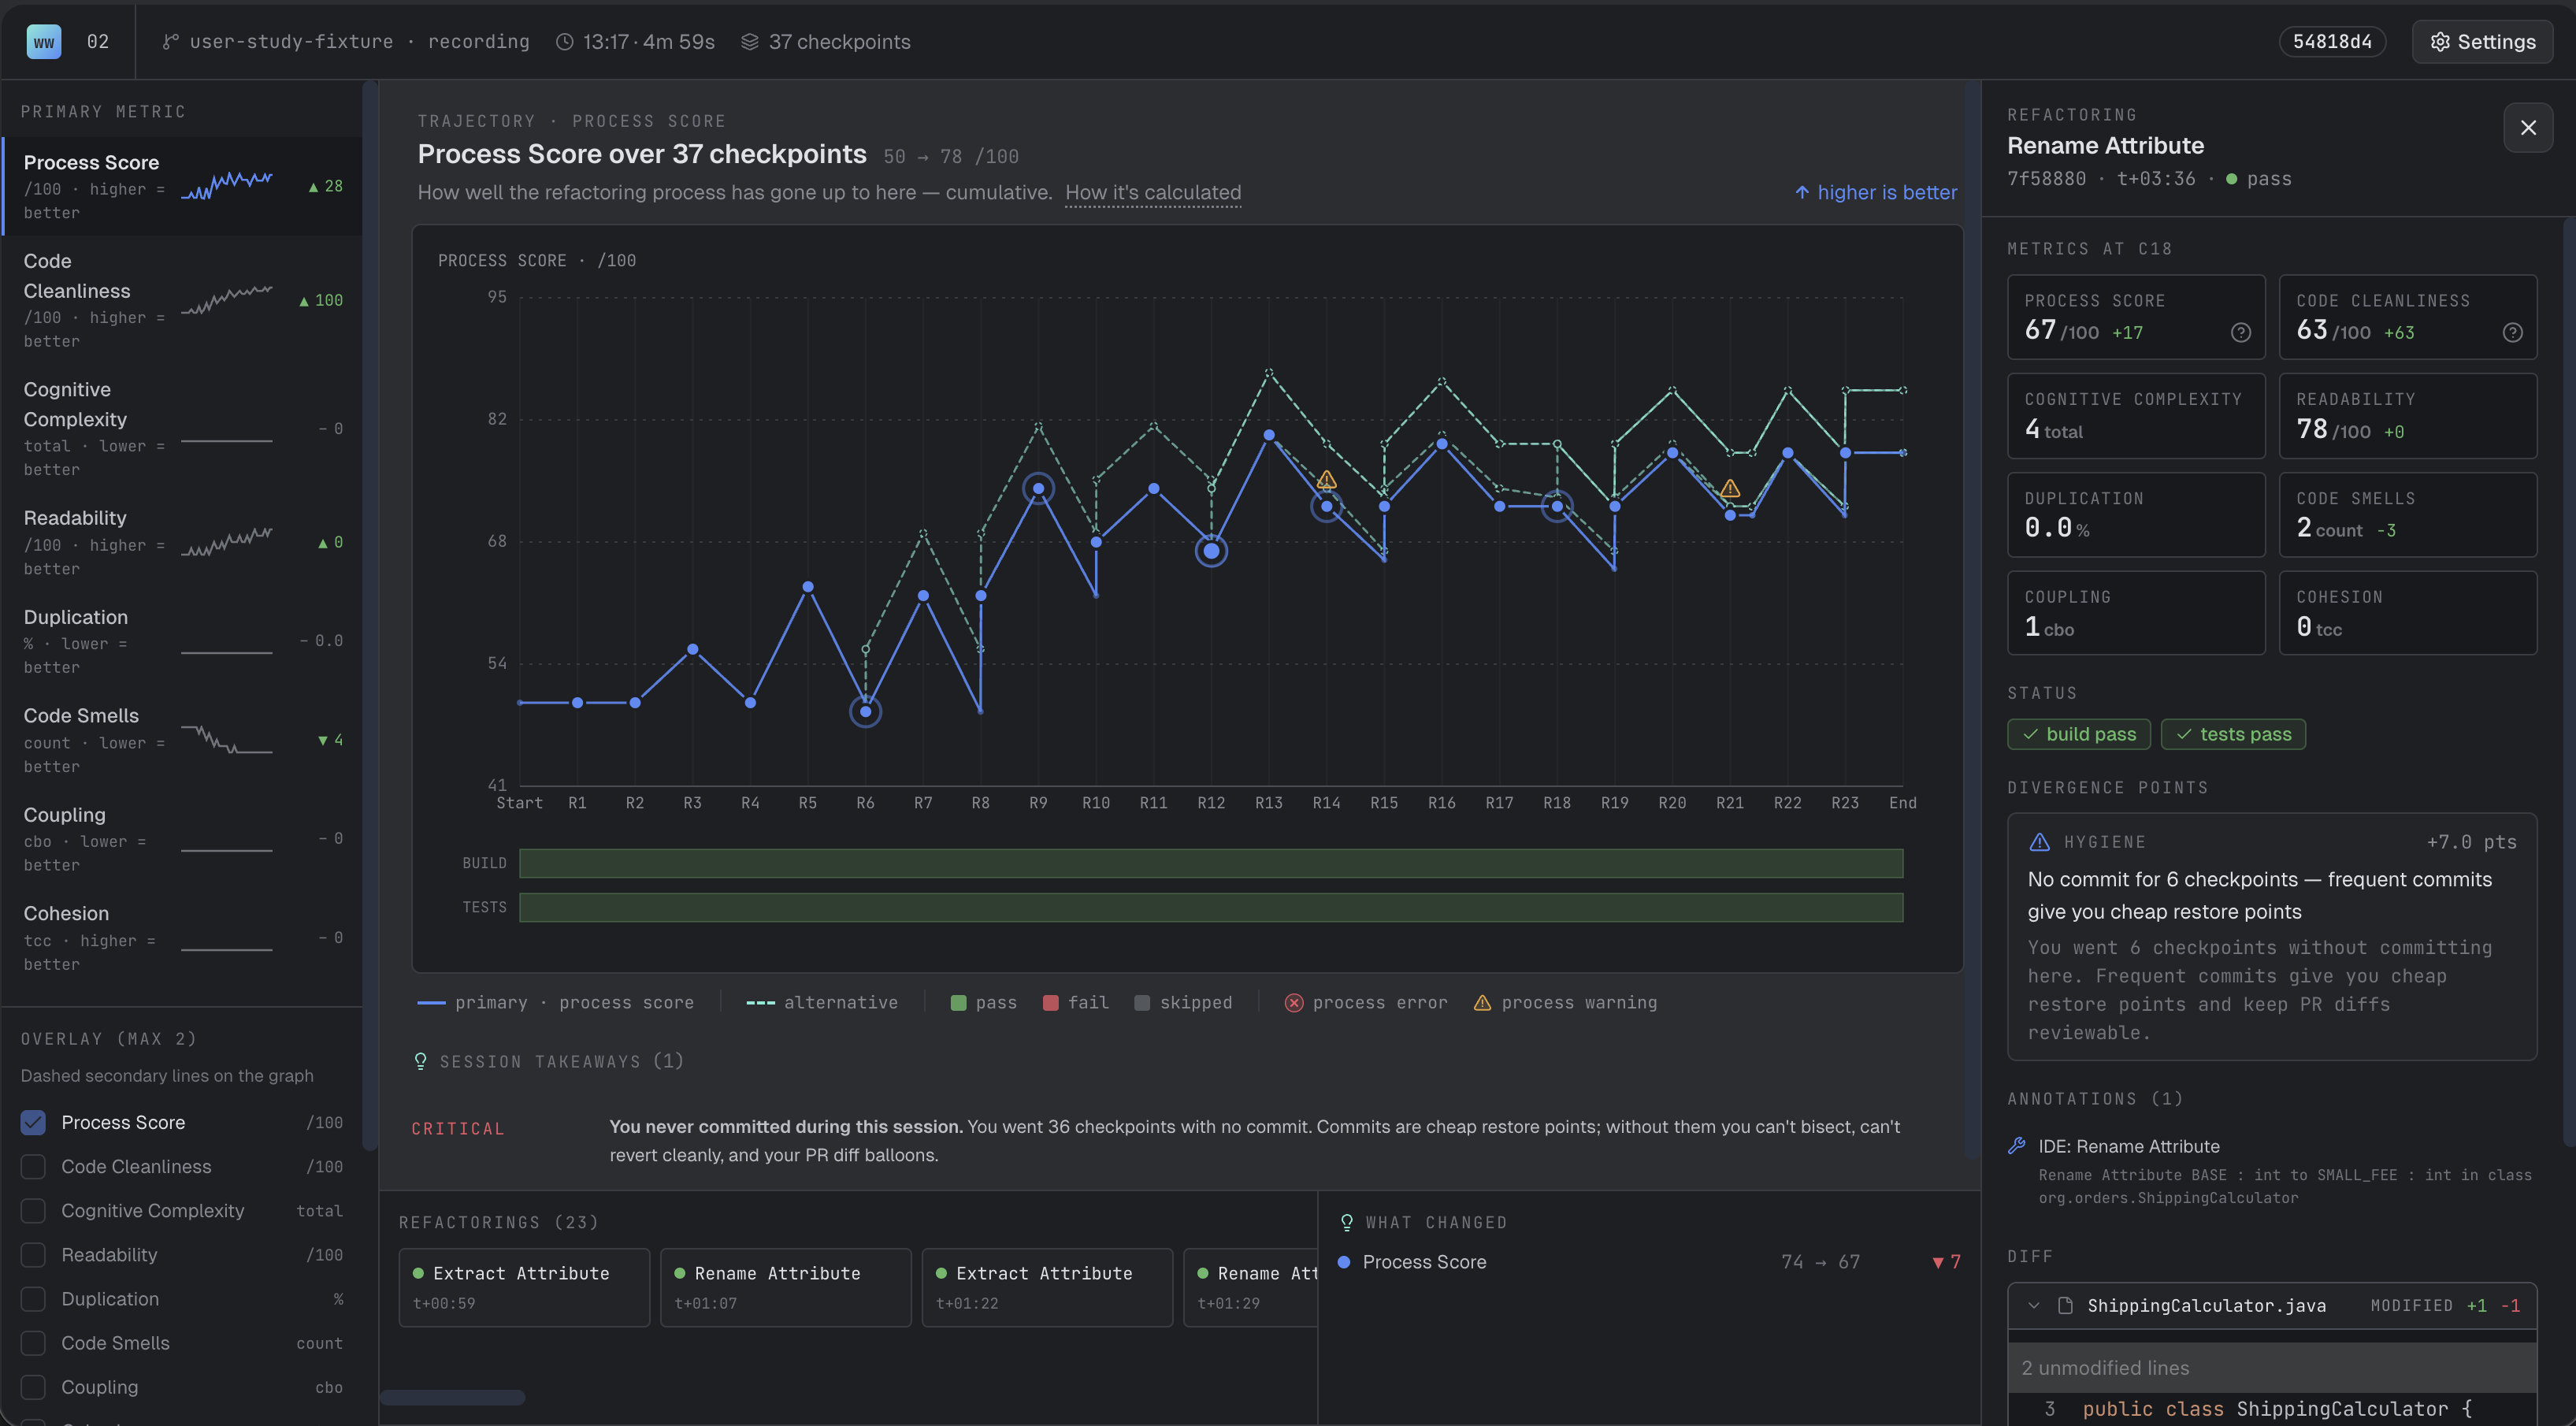
\includegraphics[width=\textwidth]{architecture/dashboard_image.png}
  \caption{The dashboard hosted inside an IntelliJ JCEF window. The centre chart plots the user's process score across the session and can overlay alternative trajectories and individual cleanliness signals. The side panels show the selected step, metric changes, build/test status, smell and duplication locations, and any divergence point associated with that step, including the suggested alternative and its score impact. The lower panel summarises the highest-impact takeaways for the session.}
  \label{fig:arch-dashboard}
\end{figure}

\section{Score-formula evaluation design}
\label{sec:methodology-score-eval}

The results chapter evaluates the score formula in two ways. The first asks whether the ranking of divergence points is stable when the weights are perturbed. The second asks whether the individual terms in the formula actually contribute to the magnitudes the detector reports. This section defines the shared experimental procedure for those tests; Chapter~\ref{ch:results} reports the observed numbers.

\subsection{Sensitivity perturbations}
\label{sec:methodology-sensitivity-design}

The sensitivity experiment compares the ranking of divergence points computed by the production weights with rankings produced under perturbed weights. Two perturbation schemes are used. In the single-knob sweep, one weight is varied while all other weights remain at their production values. In the multi-knob sweep, all weights are varied at once by drawing independent log-normal scale factors. For weight $W_i$, the sampled value is
\[
W'_i = W_i \cdot \exp(\sigma Z_i),
\]
where $Z_i \sim \mathcal{N}(0, 1)$ and $\sigma = \ln 2$. This makes the perturbation symmetric in log-space: multiplying and dividing by the same factor are treated as equally large changes, and most samples remain within a few multiples of the production value.

Ranking stability is measured with Kendall's $\tau$-b~\cite{kendall1948rank,agresti2010ordinal} and top-$N$ hit rate. Kendall's $\tau$-b is used because the rankings are short and may contain ties. A value of $\tau = 1.0$ means the perturbed ranking is unchanged, while $\tau < 0$ means the order has mostly inverted. Top-$N$ hit rate asks how many of the production top-$N$ divergence points remain in the perturbed top-$N$. Top-$1$ is the main comparison because it is defined for any session with at least one divergence point; larger $N$ values are only informative for sessions with enough surfaced points. Ties are broken by ascending step index so that production and perturbed rankings are compared deterministically.

\subsection{Ablation design}
\label{sec:methodology-ablation-design}

The ablation experiment tests whether the score formula depends on each of the seven non-sub-cleanliness terms: gain, broken-build time, skipped tests, manual-when-IDE, length, lag, and commit gap. It enumerates subsets of these process weights, keeps the selected terms at their production values, and sets the others to zero. Since there are seven non-sub-cleanliness terms, the full power set contains $2^7 = 128$ variants, which is small enough to enumerate exactly. This follows the same logic as composite-indicator sensitivity analysis~\cite{saisana2005composite} and exact Shapley-style feature attribution when the number of features is small~\cite{lundberg2017shap,strumbelj2014explaining}.

Two recovery measures are used to describe how much divergence-point magnitude remains under an ablated formula. Mean recovery computes the recovery ratio per fixture and averages those ratios. Sum-over-sum recovery instead sums $\lvert\mathrm{magnitude}\rvert$ across all divergence points in all fixtures and divides by the same sum under the production formula. Sum-over-sum is treated as the main measure because it avoids giving empty or near-empty fixtures the same weight as fixtures with many surfaced divergence points. The ablation also reports Kendall's $\tau$-b so that magnitude loss and ranking change can be considered separately.

\section{Evaluation dataset and labelling protocol}
\label{sec:methodology-rater}

The experiments in Chapter~\ref{ch:results} use a set of $45$ refactoring sessions that we recorded by hand on a Java library-style fixture in IntelliJ. This section explains how the sessions were assembled, how they were labelled, and how the labels were checked by raters.

The IDE-event capture literature surveyed in \S\ref{sec:process-aware-logging} shows that detailed development traces can be collected. However, we did not find an existing dataset that combines per-event code content with IDE-side refactoring events for Java sessions recorded in IntelliJ. This matters for the IDE-versus-manual signal. RefactoringMiner can recover a structural refactoring from a pair of code states, but it cannot tell whether the developer used the IDE refactoring command or typed the change by hand. Since that distinction is part of the manual-when-IDE penalty in \S\ref{sec:methodology-score}, it has to be captured at recording time.

The evaluation also needs controlled examples of the behaviours the detector is meant to find. The precision and recall results in \S\ref{sec:results-divergence} are computed against sessions where a specific process issue was deliberately introduced. A free-form session dataset would not provide that controlled injection signal directly. For these reasons, we recorded our own dataset using the IntelliJ plugin described in \S\ref{sec:arch-events}, so that IDE events were captured as the sessions happened.

\subsection{The 45-session injection set}
\label{sec:methodology-injection-set}

Each session follows a scripted playbook scenario designed to trigger one specific kind of process issue. Examples include choosing a less favourable order for a set of refactoring steps, undoing and redoing the same chunk of code, skipping the expected test cadence, or making a manual edit where an IDE refactoring would have applied. The playbook covers all four divergence kinds: $5$ sessions target ordering, $9$ target rework, $13$ target hygiene, and the remaining sessions are split between IDE-replay injections and clean controls where no issue is deliberately introduced.

\subsection{Two label streams}
\label{sec:methodology-labels}

Each session has two kinds of label, because the evaluation asks two slightly different questions. The first label records the divergence kind that was deliberately injected into the session, i.e. the behaviour the playbook was designed to trigger. This is used for the \emph{injection prominence} analysis in \S\ref{sec:results-divergence}. The second label is a separate hand-written set of all divergence kinds that should be detected in the session. This label can contain more than one kind, because a session designed to trigger one issue may also legitimately contain another. The per-kind precision and recall results in \S\ref{sec:results-divergence} use this second label set, and its inter-rater agreement is reported in \S\ref{sec:results-kappa}.

The multi-label schema uses the four divergence kinds $\mathcal{K} = \{\emph{IDE-Replay}, \emph{Rework}, \emph{Hygiene}, \emph{Ordering}\}$ and each session is allowed to have more than one expected kind. For example, a session may contain both an ordering divergence and a hygiene flag.

\subsection{Rater protocol}
\label{sec:methodology-rater-protocol}

To check the schema independently, two annotators, denoted P1 and P2 in the results chapter, labelled all $45$ sessions using the same schema. They completed this labelling before either of them took part in a user-study session. Each rater received the schema definition and the raw artefacts for every recording: the event log \texttt{events.jsonl} and the session metadata \texttt{session.json}. They did not receive the playbook prompts, our \texttt{manifest-v2.csv} labels, the Phase A \texttt{analysis-report.json}, or access to the dashboard. This kept the hand labels separate from both the injected labels and the detector output.

The event log stores the full file contents after each event rather than a compact diff. To make the sessions easier to inspect, raters were also given a small read-only helper script, \texttt{tool/scripts/session-event-diffs.py}, which prints a unified diff for each \emph{edit\_burst} and \emph{refactoring\_finished} event. The script is only helps to present the information from the events to the users in a more readable format and does not expose any extra information: it derives its output from the same \texttt{events.jsonl} file already given to the raters.

\subsection{Cohen's $\kappa$ computation}
\label{sec:methodology-kappa}

Agreement is reported with Cohen's $\kappa$~\cite{cohen1960kappa}, computed separately for each divergence kind in $\mathcal{K}$. For a given kind $k$, each session is treated as a binary judgement: either $k$ is present in \texttt{expected\_kinds}, or it is not. This gives a $2 \times 2$ table for each rater pair, from which $\kappa$ is computed. The results are interpreted using the Landis and Koch thresholds~\cite{landis1977kappa}: $\kappa < 0.20$ is slight agreement, $0.21$--$0.40$ fair, $0.41$--$0.60$ moderate, $0.61$--$0.80$ substantial, and $0.81$--$1.00$ almost perfect. Because the dataset contains only $45$ sessions, the raw agreement counts from each table are reported alongside $\kappa$; at this size, the yes/yes, no/no, and disagreement counts are still useful to inspect directly.

\subsection{Treatment of disagreements}
\label{sec:methodology-disagreements}

Disagreements are reported as part of the study rather than resolved by changing our labels or the raters' labels. When both raters agree with each other but disagree with our label, as with rework in session 043, the session is named explicitly in the results chapter and treated as a case where our label may be the outlier.

The rater-study results, including the per-kind $\kappa$ values, raw agreement counts, and disagreement patterns, are reported in Table~\ref{tab:results-userstudy-kappa} (\S\ref{sec:results-kappa}).

\subsection{Divergence-detector evaluation protocol}
\label{sec:methodology-detector-eval}

The divergence-detector experiment runs the full analysis pipeline on each of the $45$ recorded sessions using the production score weights. For each session, the detector output is compared with the session's \texttt{expected\_kinds} label. A true positive means that the detector surfaced at least one divergence point of the expected kind somewhere in the session, a false negative means that an expected kind was not surfaced, and a false positive means that the detector surfaced a kind not present in \texttt{expected\_kinds}. Matching is done at the session level rather than against an exact recorded step, because step boundaries depend on the plugin's edit-burst flushing and are not stable enough to treat as ground truth.

Precision and recall are reported separately for each kind. They are not collapsed into F1 or accuracy because the two error types have different practical meanings: a false positive shows the user an alternative that should not be there, while a false negative means the dashboard missed a useful opportunity. Accuracy is also uninformative because most kind-by-session cells are true negatives.

The experiment also checks whether the detector's output would be useful to a user. The first check is whether a surfaced alternative genuinely beats the user's trajectory, using the strict condition $\mathrm{magnitude} > 0$ under the trajectory-final score definition in \S\ref{sec:methodology-detector}. The second is injection prominence: for the divergence kind deliberately introduced by the playbook, the experiment records whether the corresponding positive-magnitude divergence point is the highest-ranked point in that session.
